\section{Hardware Design}

The Micromouse hardware was developed as a compact embedded system that integrates power supply, sensing, actuation, computation, communication, and user interaction on a single custom PCB. The purpose of this hardware platform is not merely to connect the required components, but to provide a reliable physical basis for closed-loop motion control and autonomous maze navigation. Since the robot operates as a mobile real-time system, the hardware design had to satisfy several requirements simultaneously: sufficient actuation power for the drivetrain, stable low-voltage supplies for the logic and sensor subsystems, low-latency access to sensor and encoder signals, and practical interfaces for programming and debugging.

At a high level, the implemented hardware can be divided into five functional blocks: the controller and timing hardware, the power-supply subsystem, the motor-drive and encoder subsystem, the infrared sensing subsystem, and the communication and user-interface subsystem. These blocks are electrically distinct, but they were designed to operate as one coordinated system. In particular, the PCB serves as the central integration platform between the battery input, the motors, the sensors, the microcontroller, and the external interfaces. This approach is advantageous in a mobile robot because it improves reproducibility, reduces wiring effort, and lowers the likelihood of intermittent connection faults that are common in loosely assembled prototypes.

Figure~\ref{fig:mouse_perspective} shows the final assembled Micromouse. The image illustrates the compact overall construction of the robot and the close integration of the mechanical platform with the electronics.

\begin{figure}[t]
    \centering
    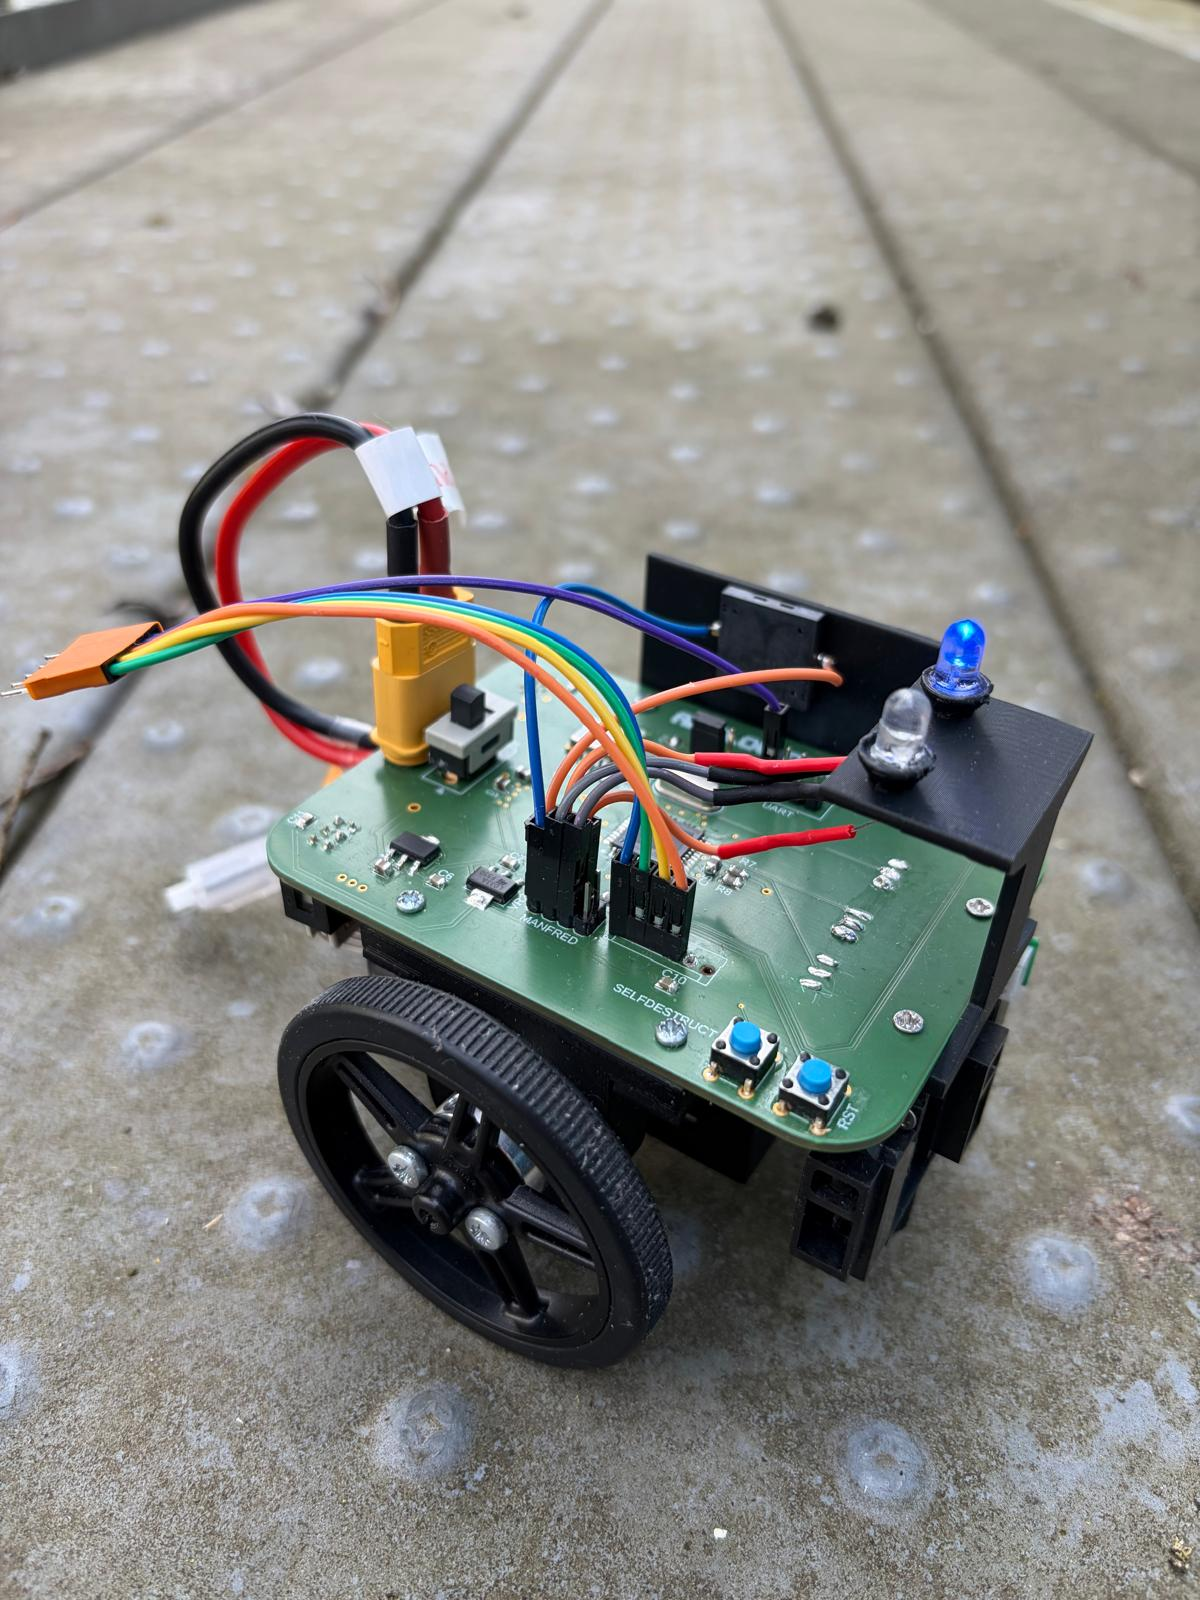
\includegraphics[width=0.85\columnwidth]{images/perspective.jpeg}
    \caption{Final assembled version of the Micromouse robot.}
    \label{fig:mouse_perspective}
\end{figure}

\subsection{Controller and Timing Hardware}

The central processing element of the robot is a \texttt{dsPIC33FJ128MC804} \cite{datasheet_dspic}. This controller was selected because it combines the peripheral functions required by the application in a single device. For the Micromouse, these functions are particularly important: PWM generation is needed for motor actuation, analogue inputs are required for the infrared sensors, quadrature encoder interfaces are needed for odometry, timers and interrupts are required for deterministic periodic execution, and UART communication is needed for debugging and monitoring. Using one controller that already supports these functions natively simplifies the circuit design and reduces the number of additional interface components.

The controller is driven by an external 16\,MHz crystal together with the associated load capacitors. This clock source provides a stable timing reference for the microcontroller and therefore supports reliable sampling, control-loop timing, and UART communication. In the firmware, the oscillator is combined with the internal PLL in order to obtain a sufficiently high operating frequency for real-time processing \cite{datasheet_dspic}. This clocking concept is well suited to the robot, because the control loop, sensor handling, and navigation logic all depend on predictable timing behaviour.

\subsection{Power Supply Architecture}

The robot is powered from a 7.4\,V battery, which forms the primary energy source of the system. From this input, the power is distributed into separate voltage domains according to the electrical requirements of the connected components. This separation is necessary because the drive system, the analogue sensors, and the digital electronics do not operate at the same supply voltage and do not have the same sensitivity to electrical disturbances.

The unregulated 7.4\,V battery voltage is used as the motor-supply domain, so that the H-bridge can provide sufficient drive voltage to the two DC motors. In operation, the effective motor drive level is limited by PWM so that the applied actuation remains compatible with the motor rating of 6\,V \cite{datasheet_motor}. A first regulator, implemented with an \texttt{LM7805}, generates a 5\,V rail \cite{datasheet_lm7805}. This 5\,V domain supplies the three infrared distance sensors and thereby provides the operating voltage for the analogue wall-detection subsystem \cite{datasheet_sensor}. From this 5\,V rail, a second regulator, implemented with an \texttt{LD1117}, generates the 3.3\,V logic supply \cite{datasheet_ld1117}. The 3.3\,V domain is used by the \texttt{dsPIC33FJ128MC804}, the \texttt{RN4871} Bluetooth module, and the remaining low-voltage digital electronics \cite{datasheet_dspic,datasheet_bluetooth}.

This staged regulation concept offers two main advantages. First, it ensures that each subsystem is operated within its intended electrical range. Second, it reduces the direct coupling of motor-related disturbances into the analogue and digital subsystems. The supporting passive components around the power stage therefore play an important role. Larger capacitors at the regulator inputs and outputs help stabilise the supply rails during load changes, while smaller decoupling capacitors placed close to integrated circuits suppress local high-frequency disturbances. Together, these measures improve the robustness of the electrical supply under the dynamic conditions of robot operation.

\subsection{Drive Electronics and Encoder Interface}

The mechanical locomotion concept of the robot is based on two independently driven DC motors in a differential-drive arrangement. Electrically, both motors are actuated through a \texttt{TB6612FNG} dual H-bridge \cite{datasheet_tb6612fng}. This component is appropriate for the project because it combines two bidirectional motor channels in one compact device and supports PWM-based control with separate direction inputs. In the implemented system, each motor is driven by one PWM signal and two logic-level direction signals, which makes it possible to realise forward motion, reverse motion, coasting, and active braking.

The motor driver is not only important for producing motion, but also for enabling controllable motion. Since the Micromouse must drive straight, execute turns, and stop repeatably, the electrical motor interface has to support both continuous duty-cycle control and rapid mode changes. The chosen H-bridge meets this requirement and integrates naturally with the PWM hardware of the dsPIC \cite{datasheet_tb6612fng,datasheet_dspic}.

Each motor is equipped with a quadrature encoder, and both encoders are connected directly to the dedicated QEI peripherals of the microcontroller. This is a particularly important design decision, because the navigation strategy depends on accurate motion feedback. The encoder signals provide the information required for wheel-speed estimation, travelled-distance measurement, and turn-progress detection \cite{datasheet_motor}. By connecting the encoders to hardware-supported quadrature interfaces, the design reduces software overhead and improves the reliability of odometry acquisition.

\subsection{Infrared Sensing Hardware}

The environmental sensing system consists of three analogue infrared distance sensors positioned to observe the left, front, and right directions. This arrangement was selected because it provides the minimum external information required by the implemented control and navigation strategy. The two side sensors are used for wall-based trajectory correction during straight motion, while the front sensor is used to detect walls ahead and to support the interpretation of cell transitions inside the maze \cite{datasheet_sensor}.

Figure~\ref{fig:mouse_front} shows the front view of the robot. This image is particularly useful because it makes the practical placement of the forward-facing sensor arrangement visible and illustrates the geometric relation between the sensor system and the maze walls encountered during operation.

\begin{figure}[t]
    \centering
    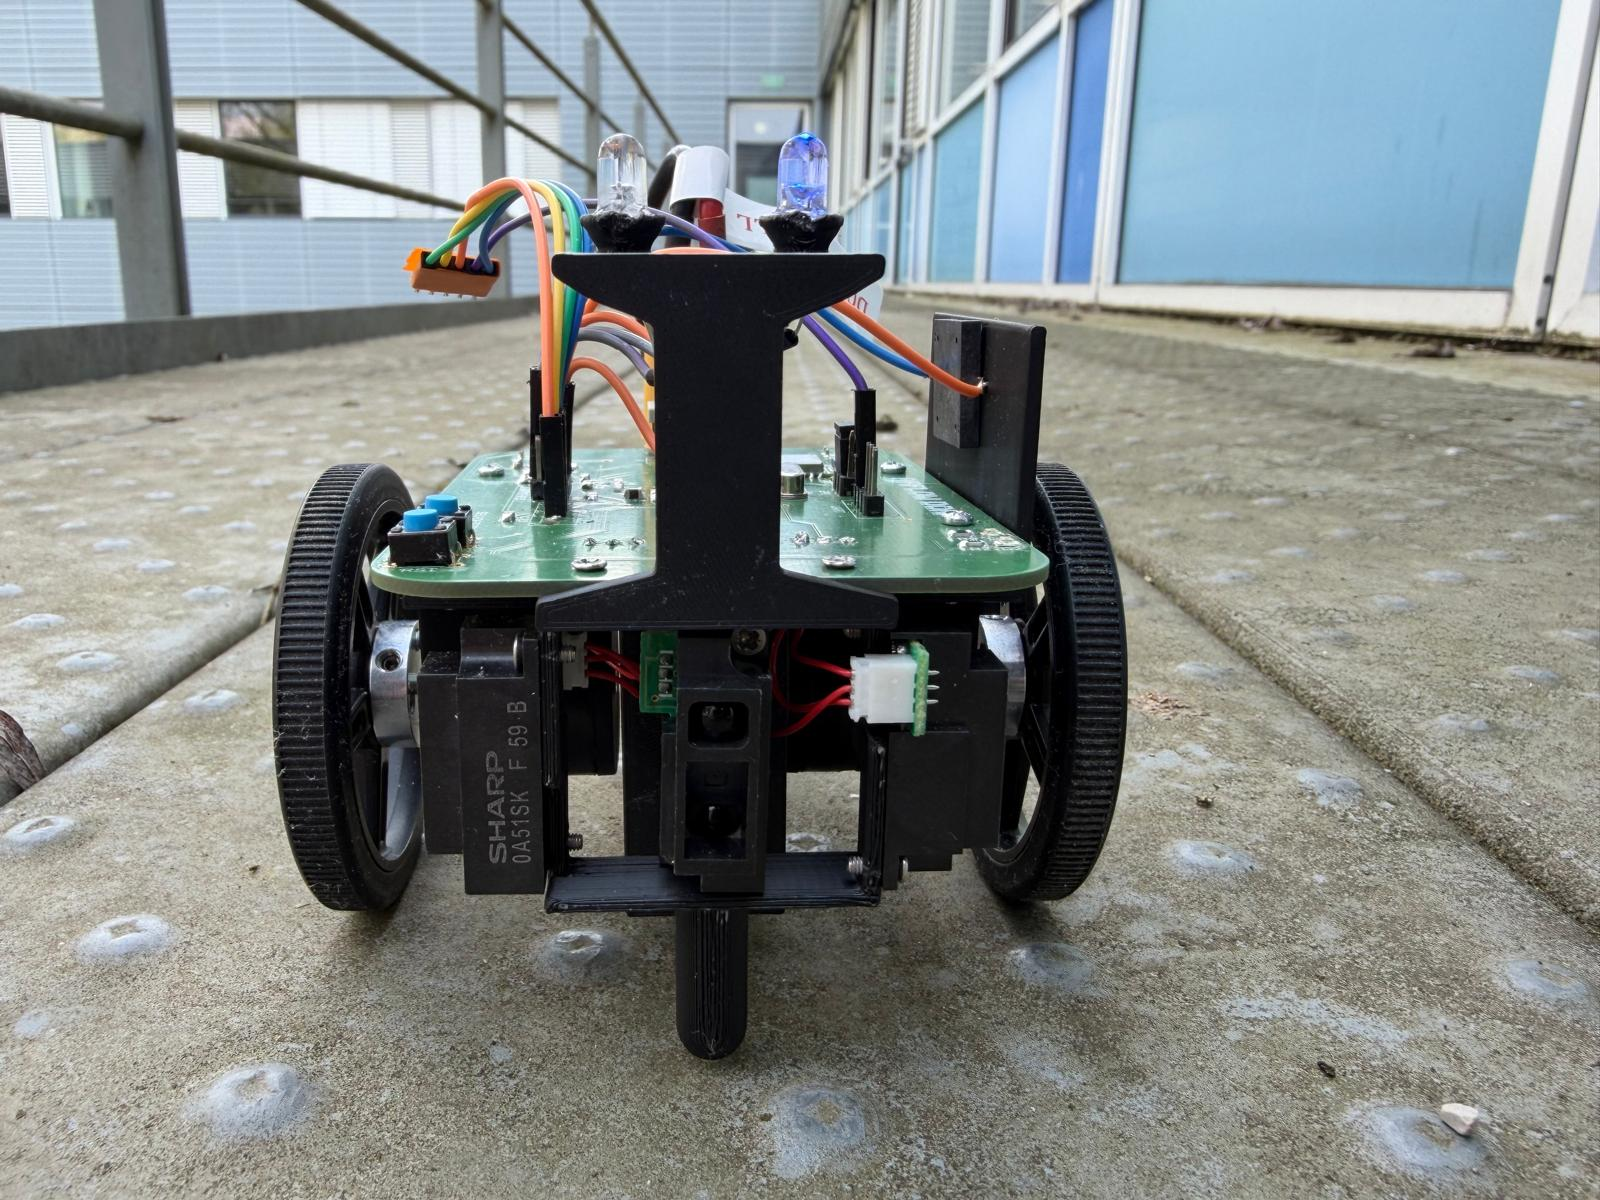
\includegraphics[width=0.72\columnwidth]{images/Front.jpeg}
    \caption{Front view of the Micromouse showing the forward sensor arrangement.}
    \label{fig:mouse_front}
\end{figure}

Electrically, the three sensors are connected to analogue inputs of the dsPIC. In the implemented pin assignment, the right, middle, and left sensors are connected to channels AN0, AN1, and AN8 respectively. The ADC is operated in 12-bit mode and scans all three channels continuously. A DMA channel transfers the conversion results directly into memory, so that recent sensor values are available without requiring the processor to handle every sample explicitly \cite{datasheet_dspic}. This arrangement is beneficial in a real-time embedded system because it combines regular sensor acquisition with low processor overhead.

The supporting analogue circuitry around the sensor inputs is comparatively simple, but still important. Since infrared wall sensing is used continuously during operation, stable sensor supply voltage and clean signal acquisition are essential. The chosen 5\,V sensor supply and the local supply-stabilisation components therefore contribute directly to measurement reliability \cite{datasheet_sensor}.

\subsection{Communication and User Interface Hardware}

In addition to the motion and sensing electronics, the robot includes dedicated interfaces for programming, debugging, and local user interaction. An ICSP programming header is provided for flashing the microcontroller during development. This interface is essential for a custom embedded board, because it gives direct access to the controller independently of the higher-level communication interfaces.

For runtime communication, the robot uses a UART interface together with an \texttt{RN4871} Bluetooth Low Energy module \cite{datasheet_bluetooth}. This module was selected as a practical wireless bridge for serial debug output. During development, this interface made it possible to observe internal variables such as sensor readings, controller states, and other diagnostic values without physically tethering the robot. For a maze-running system, this is particularly convenient because a wired connection would restrict the motion of the platform and complicate testing.

The user-interface hardware consists of push buttons and several status LEDs. The buttons provide local control functions such as start, reset, and operation changes, while the LEDs provide direct visual feedback during commissioning and testing. In practice, these simple components proved highly useful because they allowed rapid confirmation of system states without requiring a Bluetooth connection or oscilloscope measurement. The LED circuits are supported by current-limiting resistors, and the button-related logic is stabilised by suitable biasing and pull-up arrangements so that defined logic levels are maintained during operation.

\subsection{PCB Realisation and Supporting Components}

The complete electronics were implemented on a dedicated PCB rather than on separate modules. This decision is important from an engineering perspective, because the PCB is not merely a mechanical carrier but the central means of electrical integration. It defines how the power input, regulators, controller, motor driver, sensors, communication interfaces, and auxiliary components interact as one system. A custom PCB also improves repeatability and serviceability, since all major electrical connections are fixed and clearly structured.

Figure~\ref{fig:pcb_board} shows the assembled PCB of the Micromouse electronics. The image illustrates the practical realisation of the integrated hardware concept and shows how the major components are concentrated on one board.

\begin{figure}[t]
    \centering
    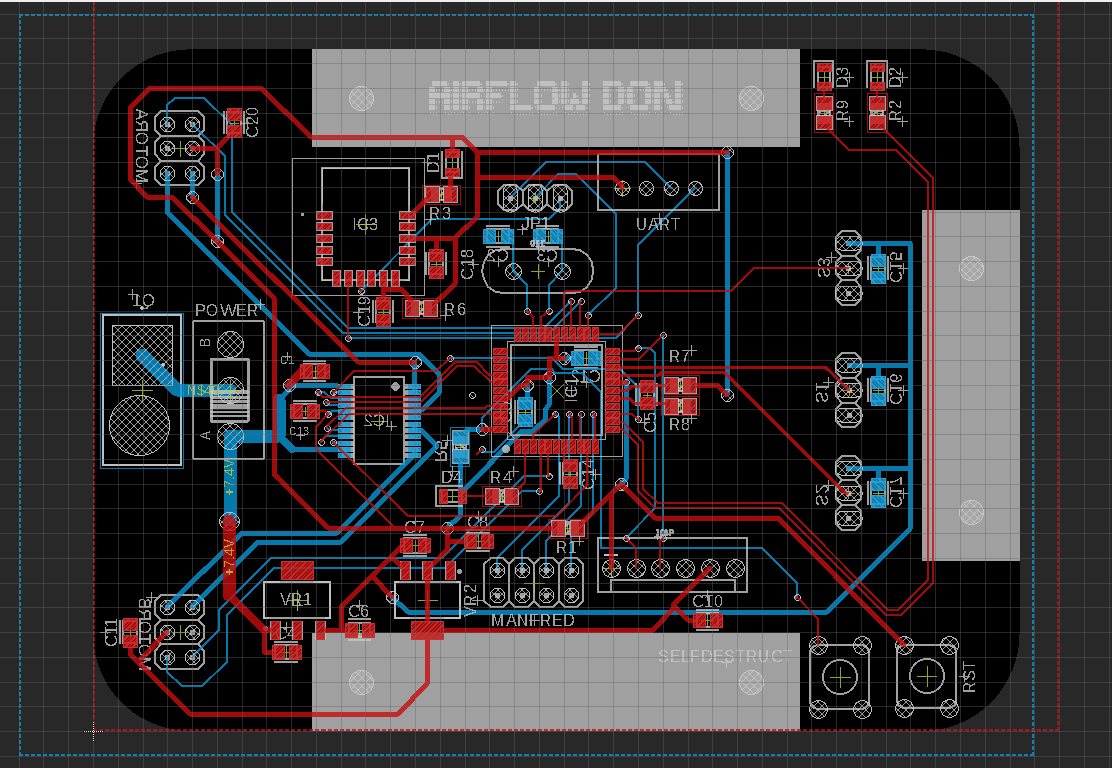
\includegraphics[width=\columnwidth]{images/board.png}
    \caption{Assembled PCB of the Micromouse electronics.}
    \label{fig:pcb_board}
\end{figure}

Besides the major active components, a considerable part of the board functionality depends on standard supporting parts. Ceramic decoupling capacitors, regulator support capacitors, crystal load capacitors, current-limiting resistors, and biasing resistors do not define the robot behaviour by themselves, but they are essential for stable operation. In particular, they ensure clean supply rails, reliable clock generation, protected LED operation, and defined logic states at sensitive inputs. For this reason, the quality of the final hardware design depends not only on the selection of the main integrated circuits, but also on the correct use of these supporting electronic components.

\section{Software Design}
The firmware was developed as a real-time embedded system that links low-level peripheral handling, closed-loop motion control, and map-based navigation. Its purpose is not only to command the motors and read the sensors, but also to maintain a consistent internal representation of the robot state while decisions are made during motion. In the Micromouse application, this is particularly important because sensing, control, and navigation cannot be treated as independent tasks: the quality of the maze map depends on accurate motion execution, while the correctness of the motion commands depends on the current navigation state.

\subsection{Software Architecture}

The implemented software follows a layered structure with three functional levels. At the lowest level, a hardware-oriented layer configures and accesses the dsPIC peripherals, including GPIO, PWM, timers, ADC, DMA, UART, and the quadrature encoder interfaces. On top of this, a driver and control layer provides reusable functions for motor actuation, encoder-based speed measurement, wall detection, Bluetooth communication, and closed-loop drive control. The highest level is the navigation layer, which stores the internal maze representation, estimates cell transitions, manages the exploration frontier, and selects the next motion command.

This separation was chosen in order to reduce coupling between tasks of different character. Hardware-specific details such as ADC configuration or PWM timing are isolated from the navigation logic, while the navigation layer operates in terms of cells, headings, and movement primitives rather than raw peripheral registers. Such a structure improves clarity and makes it easier to test and modify individual subsystems during development.

\subsection{Execution Model and Timing}

After power-up, the firmware performs a defined initialization sequence in which the clock, I/O pins, communication interfaces, timers, PWM hardware, motor and encoder interfaces, ADC with DMA support, and the controller state are configured before exploration begins \cite{datasheet_dspic}. After this initialization, the main loop remains empty and the system operates primarily in an interrupt-driven manner.

The central periodic task is executed every $10\,\mathrm{ms}$ by a timer interrupt. In this interrupt, the controller update is executed and the exploration logic checks whether the robot has reached the center of the next cell. This design was selected because both control and navigation depend on a deterministic update interval. Continuous infrared sampling is handled separately by the ADC and DMA hardware, so that current sensor values are always available in memory without requiring the processor to manage every conversion directly. In addition, encoder feedback is acquired via dedicated hardware peripherals, which reduces processor load and improves the reliability of motion estimation. A second timer interrupt is used for auxiliary functions such as audio signalling and visual feedback, but it is not part of the core navigation loop.

\subsection{State Representation and Maze Model}

The navigation layer maintains a central software state that contains the current cell position, the current global heading, the distance travelled since the last detected cell center, and the exploration status of the maze. The maze itself is represented as a $6 \times 6$ cell grid. For each cell, the software stores which neighboring cells are reachable and whether the cell has already been explored. This representation is intentionally simple, but it is sufficient for the reduced project scope because the maze can be treated as a graph of connected cells.

In addition to the maze map, the software stores temporary path information and a frontier data structure for cells that still need to be visited. This frontier is implemented in a queue-like container but operated in a Last-In-First-Out manner, so that it behaves like a stack in practice. This gives the exploration behavior a depth-first character, while still allowing the robot to compute a route through already known cells when the next target is no longer directly adjacent.

\subsection{Detection of Cell Centers}

A reliable estimate of the cell center is essential for maintaining consistency between the physical robot position and the internal maze coordinates. If a new navigation decision is triggered too early or too late, the stored map and the real robot location diverge. For this reason, cell-center detection is treated as a dedicated software function rather than as an implicit consequence of motor timing.

The implementation uses two complementary criteria. First, the travelled distance is estimated continuously from the encoder information, and a new cell is assumed once approximately one cell length has been covered. Second, the front infrared sensor is monitored during straight driving. A sufficiently strong front-wall reading can also trigger the next exploration step, since the wall geometry provides an additional indication that the robot has reached the relevant point within the cell. In this way, the software combines odometry-based estimation with environmental sensing in order to reduce the risk of losing orientation.

\subsection{Exploration Strategy and Direction Handling}

At the beginning of a run, the software initializes the robot with a start position, a start heading, and an empty maze map. The start cell is marked as explored, and the first candidate target cells are inserted into the frontier structure. Whenever the robot reaches a new cell center, the software evaluates the left, right, and front wall sensors relative to the current robot heading. Each detected open direction is then converted from the local frame of reference into the corresponding global maze direction and stored as a valid neighbor connection in the map.

This distinction between local and global orientation is central to the software design. Locally, the robot reasons in terms of front, left, right, and rear because this matches the sensor arrangement and the available turning commands. Globally, however, the maze must be stored consistently in terms of north, east, south, and west. The navigation logic therefore includes an explicit transformation between both representations. This ensures that sensor observations made from different robot headings can still be integrated into one coherent map.

\subsection{Path Selection and Goal-Directed Operation}

After updating the map of the current cell, the software determines the next target. If the next frontier entry is directly adjacent, the required action can be derived immediately as a local movement decision. If the target lies elsewhere in the already explored part of the maze, the software computes a path through the known map by recursively searching through the reachable neighboring cells and selecting the shortest currently known route. The resulting sequence of global directions is then executed step by step by combining turning primitives with straight motion.

The overall navigation behavior is divided into two phases. In the first phase, the robot explores the accessible maze and constructs the map incrementally. Once no unexplored frontier cells remain, exploration is marked as complete and the robot uses the stored map to return to the start region. In the second phase, triggered separately by the user, the robot calculates a path from its current position to the predefined goal and follows this route through the known maze. This two-phase structure was chosen because it separates map generation from map exploitation and thereby makes the system behavior easier to test and interpret.
